\section{Methodology}
\label{sec:methodology}

% Architectural Overview. Begin with High-Level Diagram and then briefly walk into the main stages. 
% Implementation and Experimental Setup is seperate section. Introduce the Research Questions here. 

This section details the methodology leveraged by \textit{EnCoDe}. It is organized into a sequence of phases, beginning with the creation of a ground-truth dataset via our novel \textit{PowerLens} measurement methodology, followed by feature extraction, and culminating in the training of predictive models. 

To further explain the methodology followed in detail, we will use the following simple running example of a  Python function (\textit{Listing \ref{lst:calculate_score}}), demonstrating how it is transformed from raw code into a final energy estimate.

\begin{listing}[ht]
\centering
\begin{tcolorbox}[
    colback=codebg,
    colframe=framecol,
    arc=5mm,
    boxrule=1pt,
    title=\textbf{Example: \texttt{score\_function.py}},
    coltitle=black,
    fonttitle=\bfseries,
    top=1mm, bottom=1mm, left=2mm, right=2mm
]
\begin{lstlisting}[language=Python, basicstyle=\small\ttfamily, breaklines=true]
def calculate_score(items, threshold):
    score = 0
    for item in items:
        if item > threshold:
            score += (item * 2)
    return score
\end{lstlisting}
\end{tcolorbox}
\caption{Example: score computation function in Python}
\label{lst:calculate_score}
\end{listing}


\begin{figure*}[htbp]
  \centering
  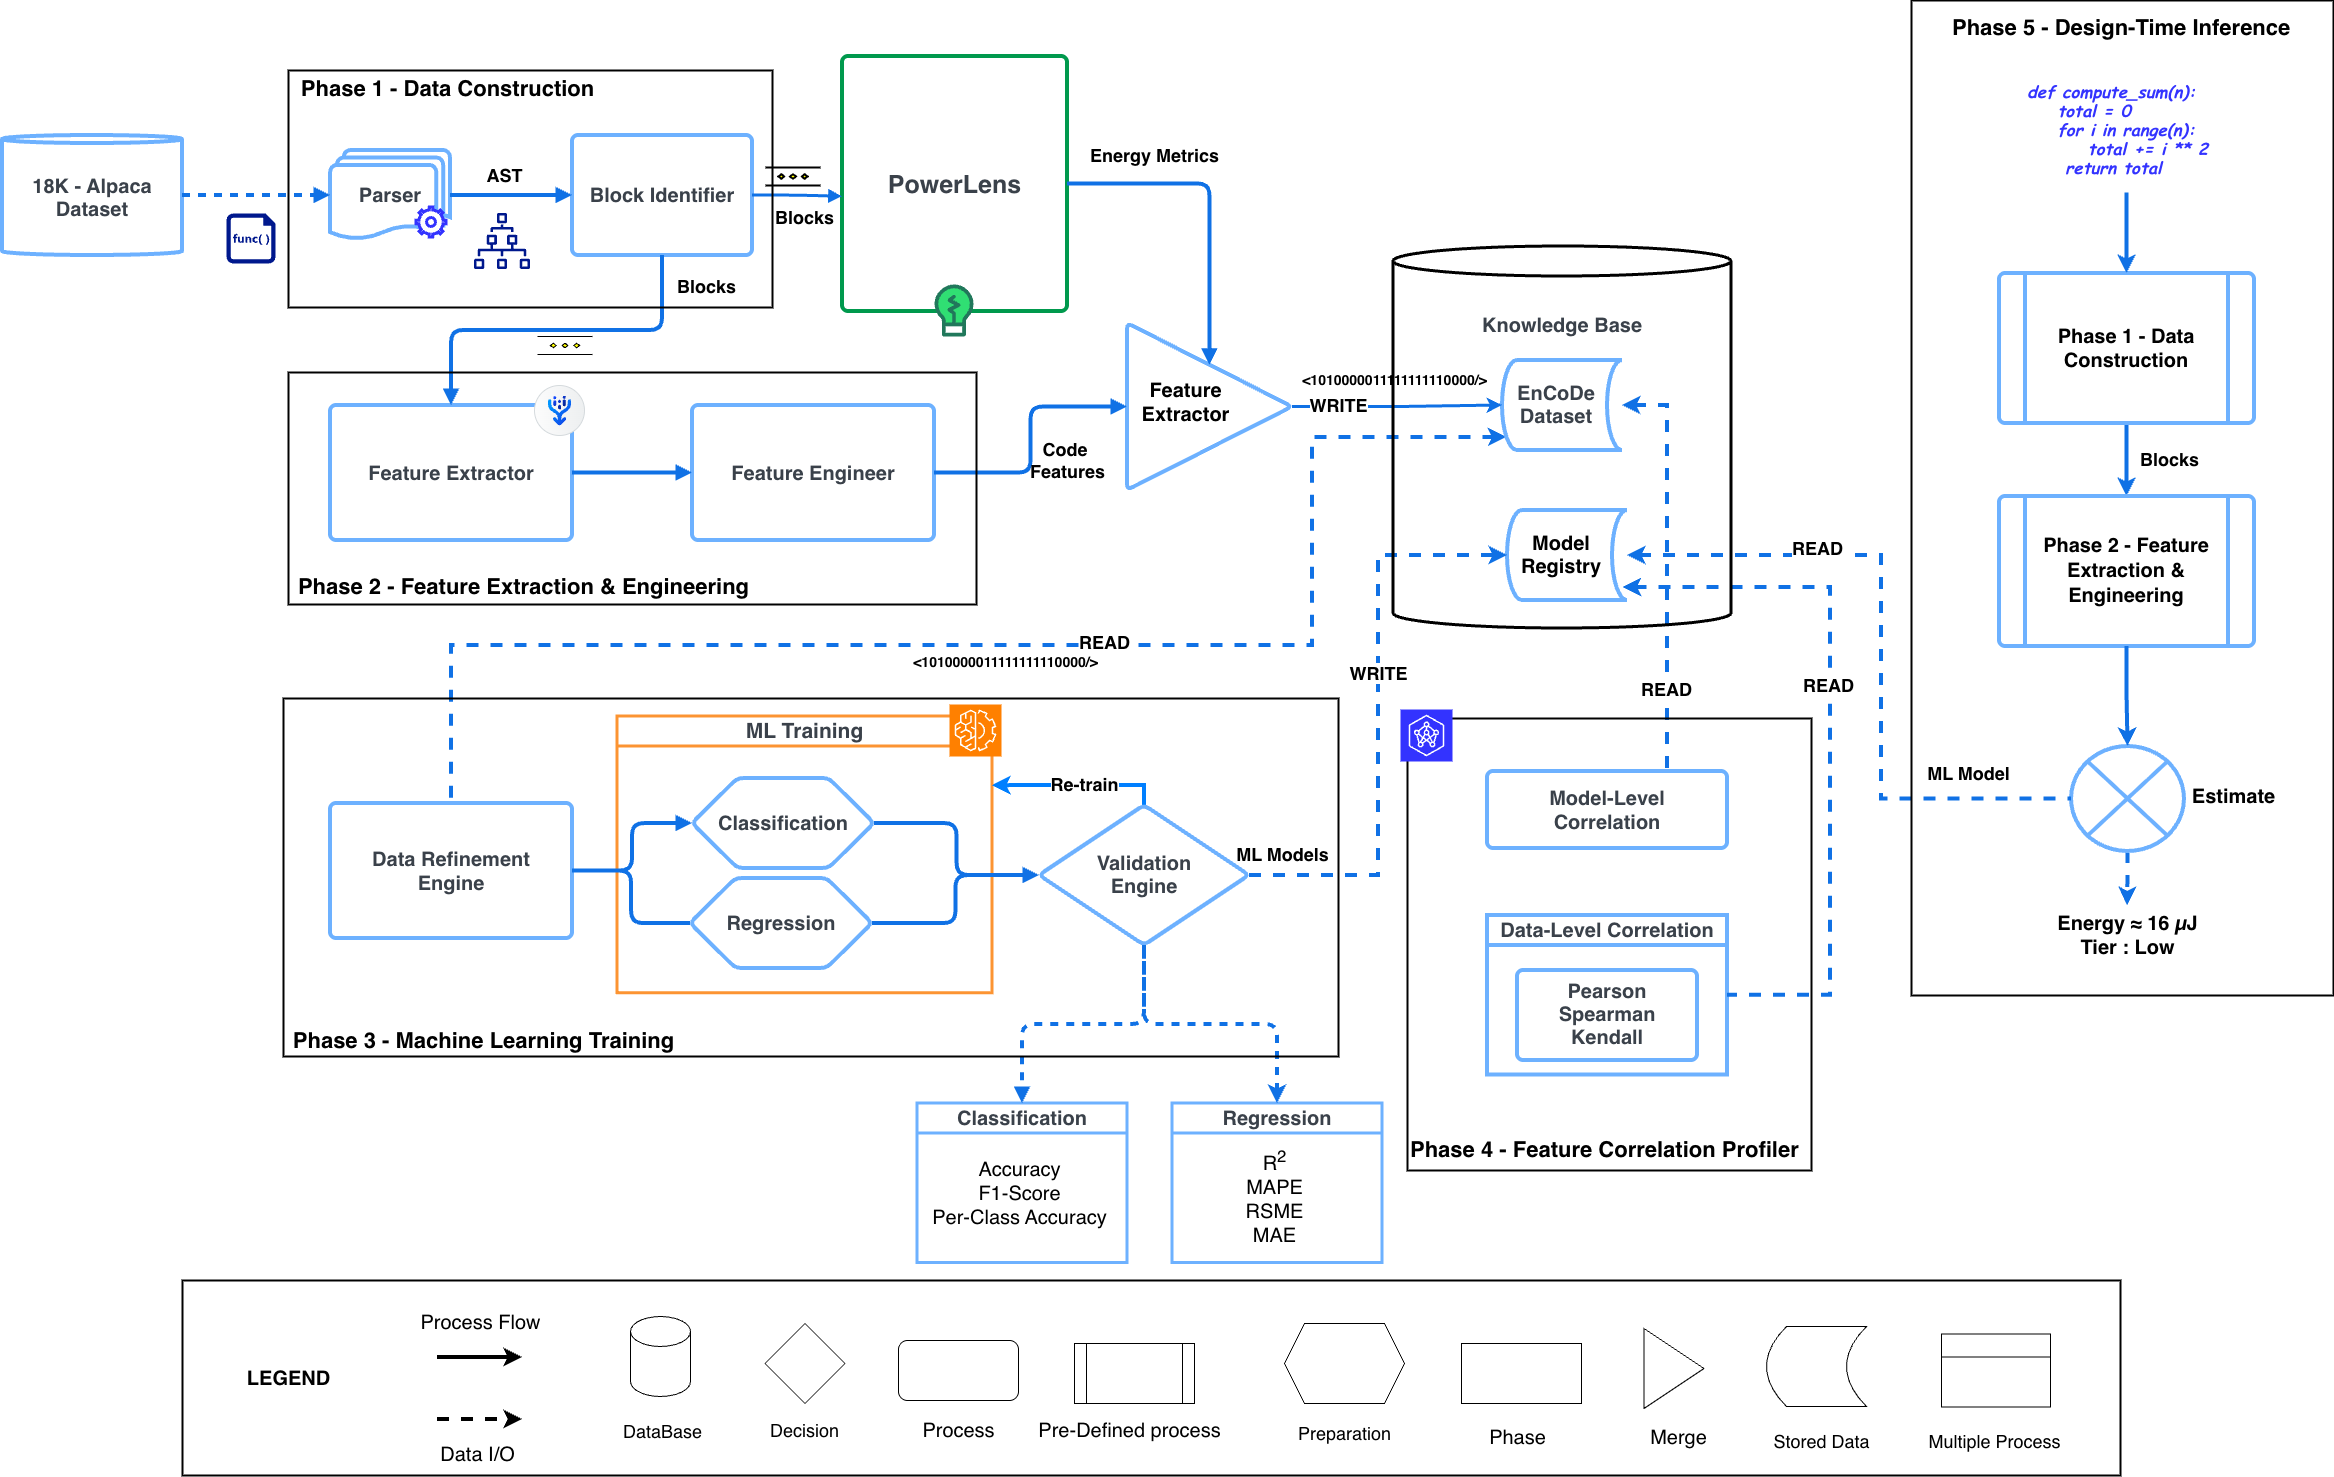
\includegraphics[width=0.95\textwidth]{figures/EnCoDe.png}
  \caption{Design Time Energy Estimation Methodology}
  \label{fig:framework}
\end{figure*}



% This function contains several distinct computational units (blocks) such as a function definition (\textit{def}), a loop (\textit{for}), and a conditional (\textit{if}), whose individual energy contributions are precisely what \textit{EnCoDe} is designed to analyze. 

\subsection{Phase 1 - Data Construction}
\noindent
The first phase of our methodology, as shown in \textit{Figure \ref{fig:framework}}, transforms a raw program text into a structured, analyzable computational block. This is achieved by first parsing the source code \(\mathcal{P}\) to its \textbf{Abstract Syntax Tree (AST)}, a hierarchical representation of the code's structure\cite{Aho1986CompilersPT, sun2023abstractsyntaxtreeprogramming}, as shown in \textit{Figure \ref{fig:block_identification}}. We then traverse the AST to identify node types that represent the root of distinct blocks. We define these block-rooting node types as:

\[ \mathcal{V}_{block} = \{FunctionDef, For, While, If, Try, With\} \]

Each node of these types, along with the entire subtree rooted at that node, is designated as a distinct block, as shown in \textit{Figure \ref{fig:block_identification}}. 

% For example, after parsing our \textit{Listing \ref{lst:calculate_score}} into its AST, this phase identifies all nodes whose types match our defined set of block-rooting nodes (\( \mathcal{V}_{block} \)). This process yields three distinct, nested blocks, each corresponding to a specific AST subtree:

% \begin{itemize}
%     \item \textbf{B0}: Root node of the AST (module level)
%       \begin{itemize}
%         \item \textbf{B1}: \textit{FunctionDef}(\texttt{calculate\_score})
%           \begin{itemize}
%             \item \textbf{B2}: \textit{For} loop inside the function
%               \begin{itemize}
%                 \item \textbf{B3}: \textit{If} statement inside the loop
%               \end{itemize}
%           \end{itemize}
%       \end{itemize}
% \end{itemize}

For \textit{Listing~\ref{lst:calculate_score}}, this yields three nested blocks: B1 (\textit{FunctionDef} \texttt{calculate\_score}), B2 (\textit{For} loop), and B3 (\textit{If} statement inside B2), preserving their containment hierarchy.

The output of this phase is a collection of AST subtrees, each treated as an atomic block. Crucially, their hierarchical context is preserved (e.g., we know B3 is nested within B2), which is essential for all subsequent measurement and feature extraction. 


\begin{figure*}[htbp]
  \centering
  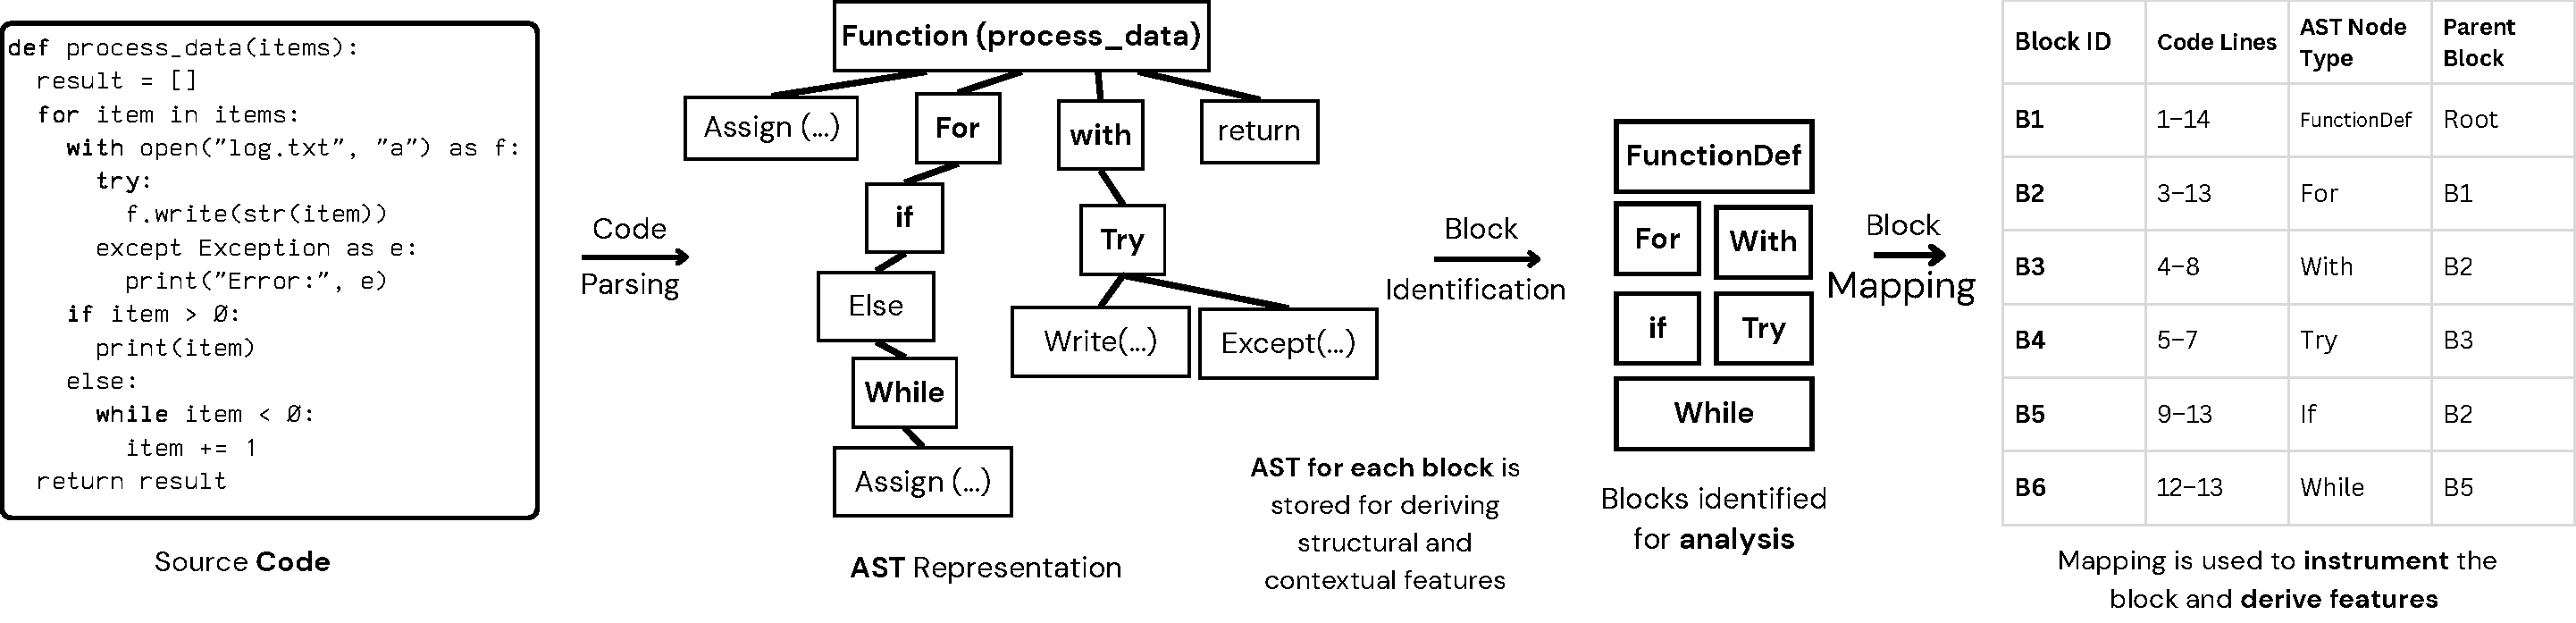
\includegraphics[width=0.95\textwidth]{figures/block_identification.pdf}
  \caption{Code Parsing to identify blocks from AST}
  \label{fig:block_identification}
\end{figure*}
\begin{figure*}[htbp]
  \centering
  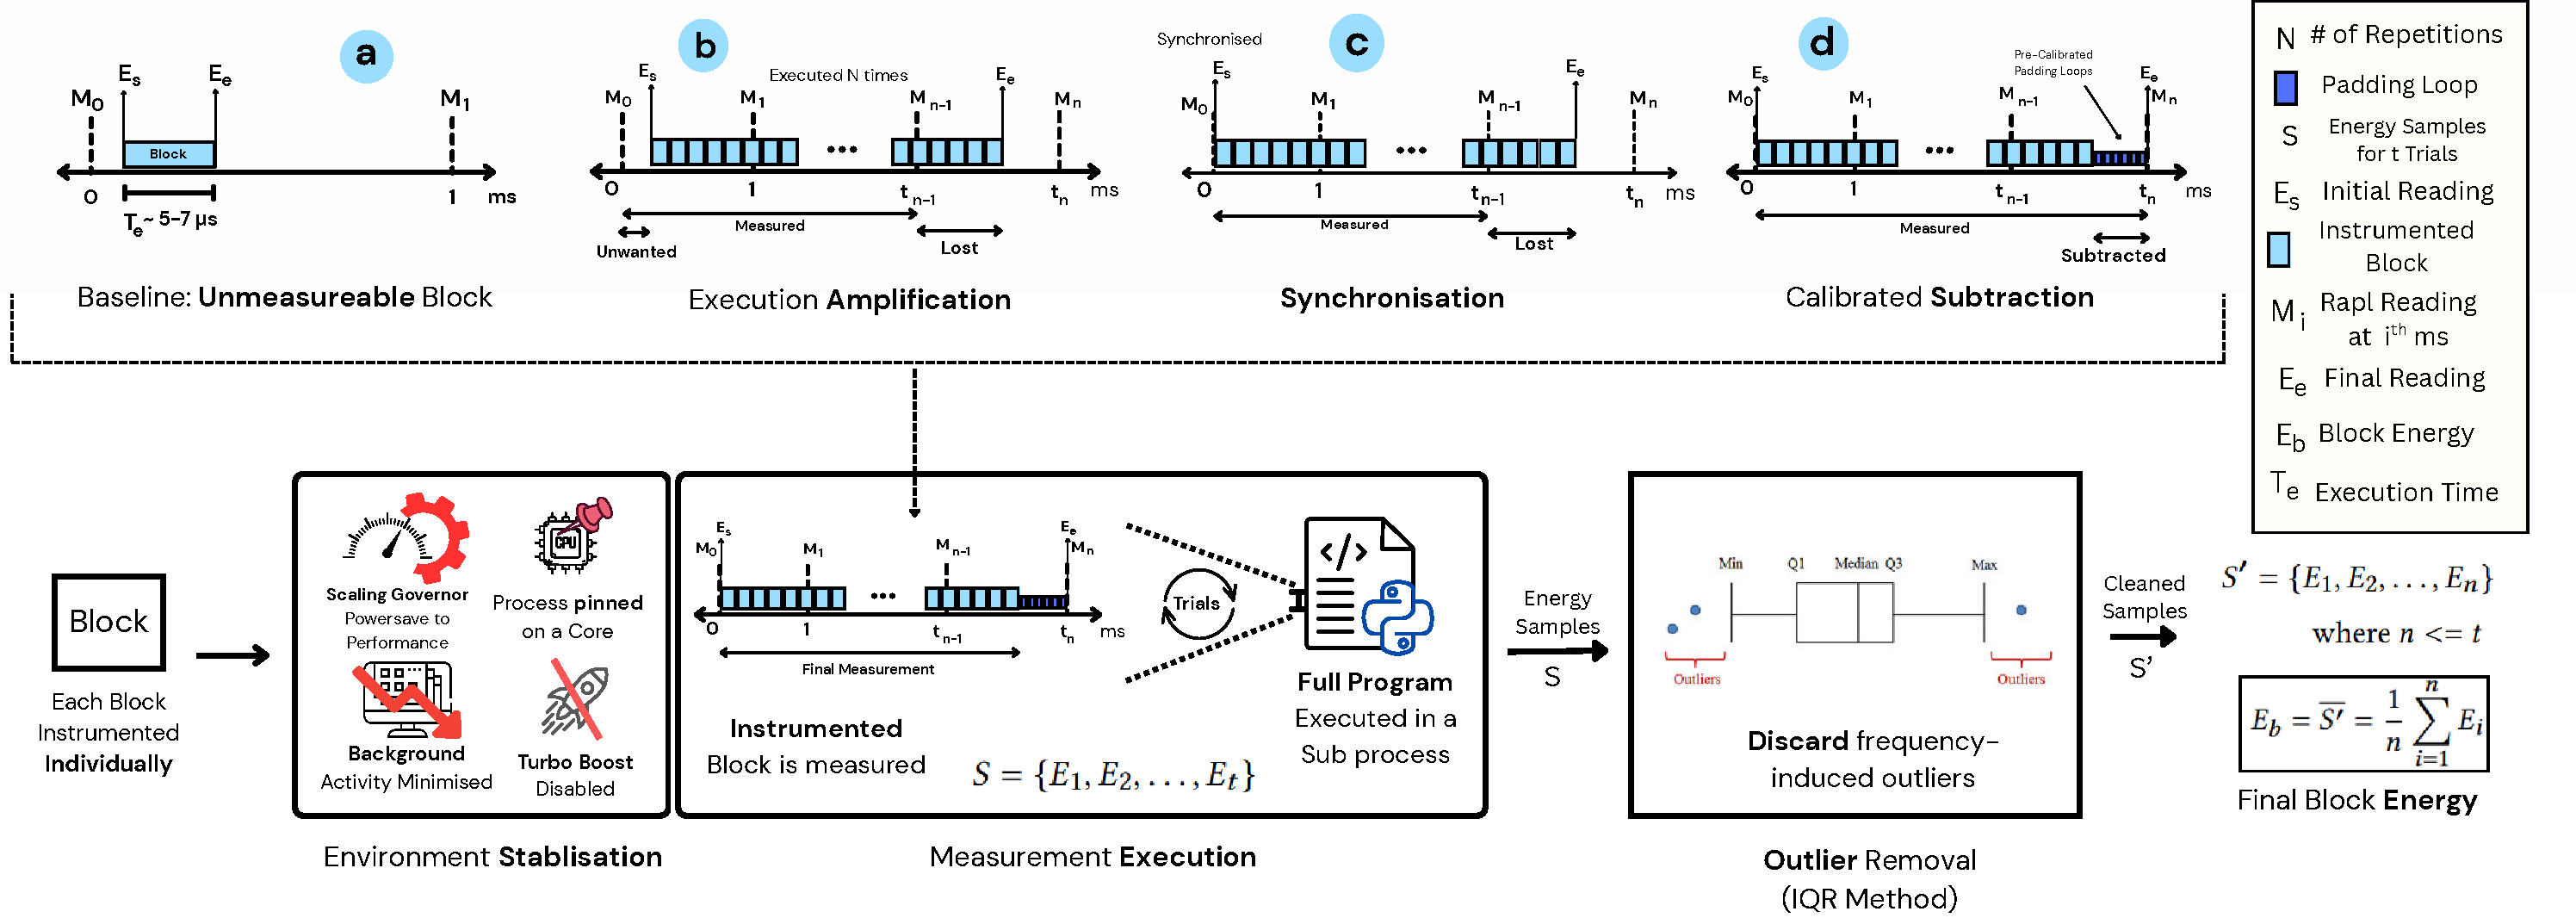
\includegraphics[width=0.95\textwidth]{figures/powerlens.pdf}
  \caption{PowerLens : Sub-Millisecond Energy Measurement Methodology}
  \label{fig:powerlens}
\end{figure*}
% \begin{figure}[t]
%   \centering
%   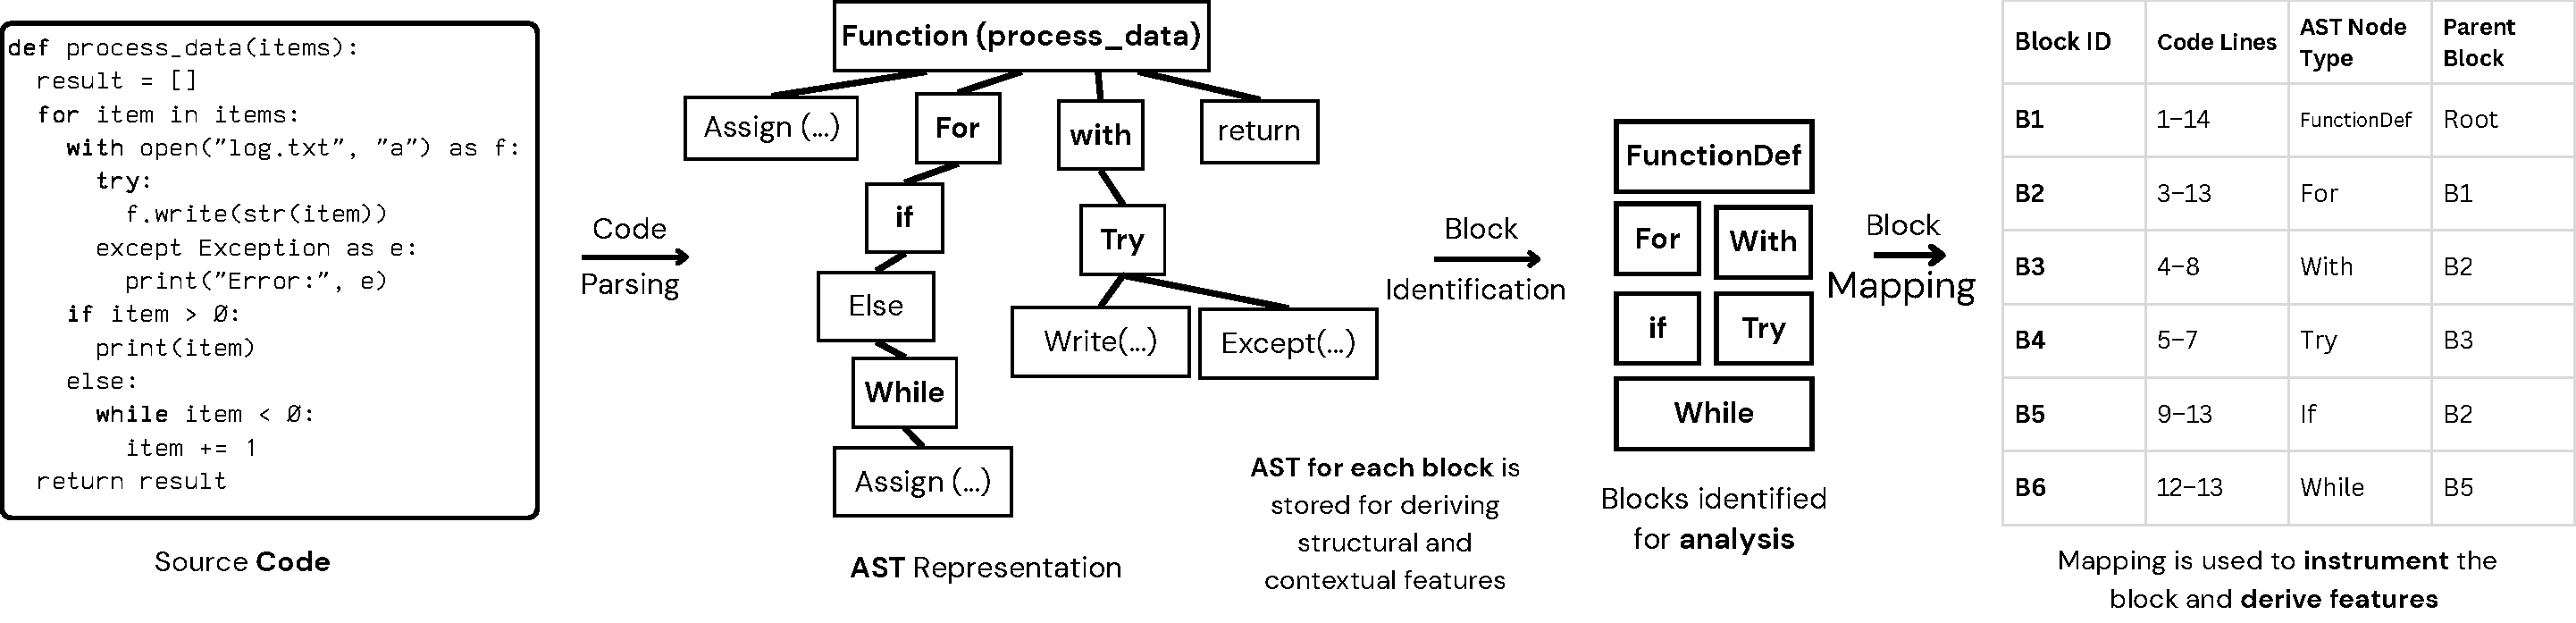
\includegraphics[width=\linewidth]{figures/block_identification.pdf}
%   \caption{Code Parsing to identify blocks from AST}
%   \label{fig:block_identification}
% \end{figure}
% \begin{figure}[t]
%   \centering
%   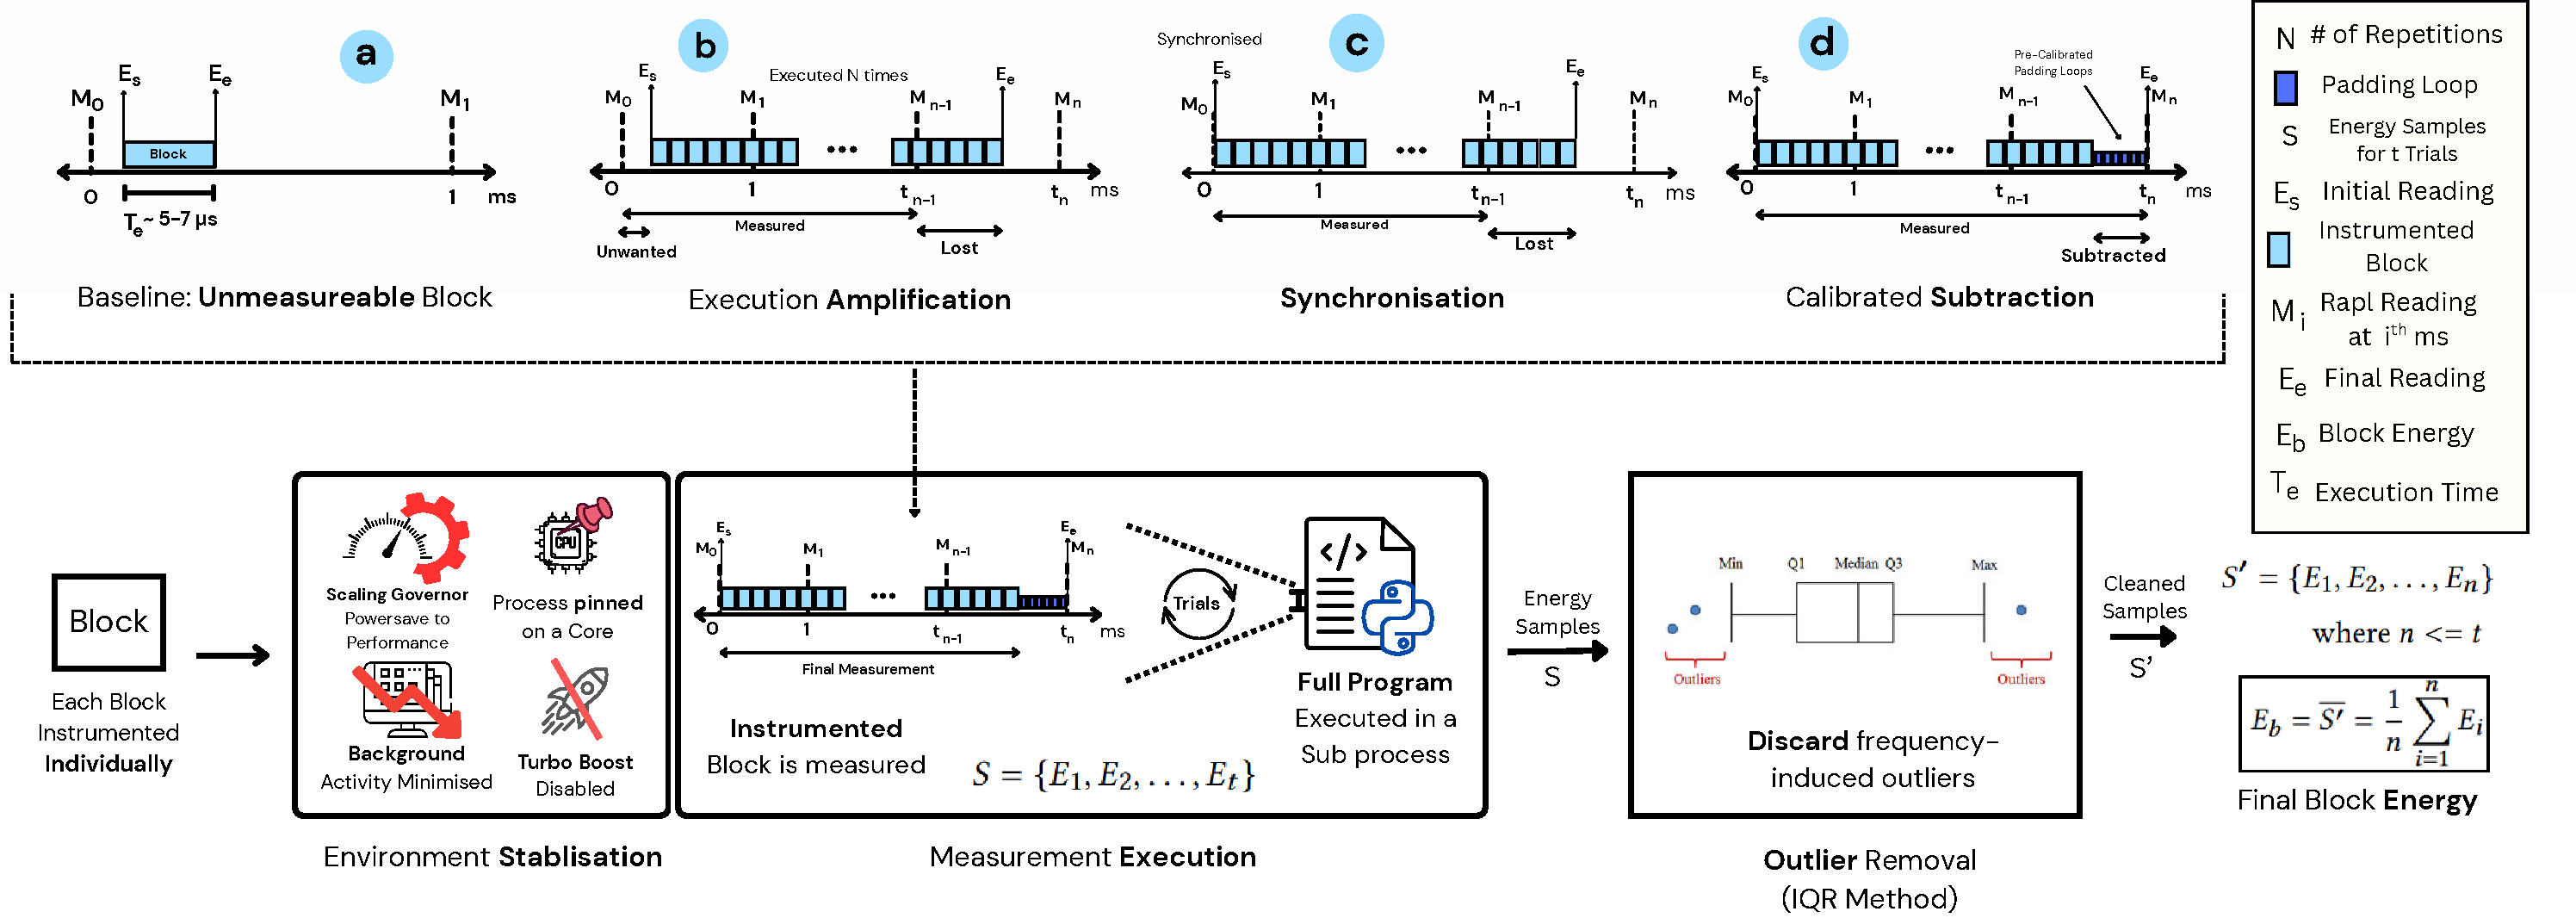
\includegraphics[width=\linewidth]{figures/powerlens.pdf}
%   \caption{PowerLens: Sub-Millisecond Energy Measurement Methodology}
%   \label{fig:powerlens}
% \end{figure}

\subsection{PowerLens: Fine-Grained Energy Measurement}

With the code blocks identified, \textit{PowerLens} measures their energy consumption to create our ground-truth dataset. This is the core technical challenge of our work: a block like the \textit{if} statement (B3) as mentioned in our phase 1, executes in microseconds, far too fast for standard hardware counters like Intel's RAPL to measure directly \cite{ 10.1145/2425248.2425252}. Existing tools, therefore, cannot provide this data, as discussed in related work. \textit{PowerLens} addresses this fundamental measurement 
problem by extending prior work~\cite{10.1145/2425248.2425252}, operating 
through four coordinated mechanisms.

\subsubsection{Environmental Stabilization}
\label{sec:enviromental_Stab}
To ensure measurements are stable, we must isolate the execution from system “noise”. Fluctuations in CPU frequency or background processes can easily distort the tiny energy signature. \textit{PowerLens} enforces a stable environment by setting frequency scaling governor to performance, disabling Turbo Boost, pinning the measurement process to a single core, and suspending non-essential background processes. This ensures that the energy we measure is attributable to the code block itself. 


\subsubsection{Execution Amplification.}

A single execution of a block like our \textit{if} statement (B3) is too fast to register on RAPL's millisecond-scale counters. To make this imperceptible signal measurable, \textit{PowerLens} wraps the target block in a tight loop and executes it \( N \) times. This amplifies the total energy consumed to a level that rises clearly above the millisecond-scale. The total energy \( E_{total} \), is calculated by taking two snapshots of the RAPL energy counter:\( (E_s) \) taken before the execution window, and \( (E_e) \) taken immediately after, as shown in \textit{Figure \ref{fig:powerlens}}. The measured difference is modeled as: 

\[ E_{total}(b, N) = E_e - E_s = N * E(b) + \epsilon_N \]

where \( E_b \) is the true energy of a single execution and \( \epsilon_N \) is the measurement noise which becomes negligible when averaged over N repetitions. By linear aggregation, the estimated mean energy per execution, \( \hat{E(b)} \), becomes:

\[ \hat{E(b)} = \frac{E_{total}(b,N)}{N} \]

For example, to measure B3 as discussed in Phase 1, we execute it N times. If the total measured energy \( E_{total} \) is \( 0.04 \) Joules (J), our initial measurement for a single execution is \( \hat{E}(B3) = 0.04 J / 1000 = 4.0 * 10^{-5} J \). 

\subsubsection{Synchronization - Aligning Execution and Sampling}

Amplification alone is insufficient. If the execution loop starts or end in the middle of a RAPL sampling window, the measurement will be corrupted by energy from unrelated computations, as illustrated by the “unwanted” energy in \textit{Figure \ref{fig:powerlens}}. To solve this, \textit{PowerLens} synchronizes the start of the execution loop with the RAPL counter's refresh cycle.  The start time \( t_0 \) is formally defined as the first moment a counter update is detected after the previous measurement start \( t_s \):

\[ t_0 = min\{ t > t_s | M_{i+1} > M_i \} \]

where \( M_i \) is the cumulative RAPL reading time at time tick \textit{i}. This precise alignment guarantees that the captured energy is attributable only to our target block. 


\subsubsection{Calibrated Subtraction}

As amplified execution rarely finishes exactly on a RAPL boundary, a small “padding” interval is needed to complete the measurement window, and this padding consumes energy that must be removed. \textit{PowerLens} subtracts a pre-calibrated energy cost for this padding, \( E_{pad}(\delta t) \), which is modeled as a linear function of the padding duration \( \delta t \). The final, net energy for a single trial is then:

\[ E_{net}(b) = \frac{E_{total}(b,N) - E_{pad}(\delta t)}{N} \]



\subsubsection{Statistical Aggregation - Achieving Reproducibility}

To ensure the final value is robust against any residual system noise (eg., transient interrupts, SMM), the entire process is repeated \(m (=10)\) times. Outliers are filtered from these trials using the standard \textit{Inter-quartile Range (IQR)} rule \cite{alma9995263502466}. The final energy signature for a block, \( \hat{E(b)} \), is  the mean of the stable, non-outlier observations:

\[ \bar{E}(b) = \frac{1}{|\Omega(b)|} \sum_{i \in \Omega(b)} E_{net}^{(i)}(b) \]

where \(\Omega(b)\) denotes the non-outlier trial set. 

This is applied independently to each block, producing reliable, ground-truth energy values: \(\{B1: 7.7e-2 J, B2: 7.5e-2 J, B3: 1.4e-6 J\}\). This data, which could not be obtained with prior software methods forms our ground truth.

\subsection{Phase 2 - Feature Extraction and Engineering}

After energy measurements, the next step is to create a numerical "fingerprint" for each block based on its source code\cite{10.1145/3639475.3640110}. The goal is to compute a set of static features that capture the block's structural and syntactic characteristics, which we hypothesize are predictive of its energy consumption. This process creates the foundation for our predictive models, as illustrated in \textit{Figure \ref{fig:framework}}.

\subsubsection{Feature Extractor}

This component operates on the AST of each block, computing a feature vector \( x_b \) composed of 33 metrics grouped into seven categories. These categories are designed to capture different facets of code: 

% \smallskip
%\begin{itemize}
\noindent \textbf{Basic Metrics (5)}: Capture the block's overall scale (e.g., AST node count, depth). These serve as a baseline proxy for the total number of components.

% \smallskip
\noindent
\textbf{Complexity Metrics (4)}: Quantify logical intricacy using measures like cyclomatic complexity\cite{1702388}. Prior studies have established a direct correlation between high complexity and increased power consumption, as it often translates to more conditional branches in the instruction stream \cite{Keong2015MetricsPower}.

% \smallskip
\noindent
\textbf{Density Metrics (5)}: Measure the concentration of computational work, such as the ratio of operators to total AST nodes. Dense code regions often correspond to higher instruction throughput and sustained CPU activity.

% \smallskip
\noindent
\textbf{Diversity Metrics (6)}: Assess the heterogeneity of code elements (e.g., entropy of operator types). High diversity may engage a wider range of CPU functional units, influencing micro-architectural energy states.

% \smallskip
\noindent
\textbf{Structural Metrics (3)}: Capture the shape of the control-flow graph (e.g., branching factor), which impacts instruction fetch and branch prediction energy costs. \cite{10.1145/3212695}

% \smallskip
\noindent
\textbf{Code Pattern Metrics (5)}: Identify the presence of semantic constructs like loops and conditionals, which are primary determinants of a block's dynamic execution behavior.

% \smallskip
\noindent
\textbf{Halstead Metrics (5)}: Model the informational complexity of code (e.g., program volume, program effort)\cite{10.5555/540137}. While designed for cognitive effort, Halstead metrics are considered key indicators of software maintainability, a crucial aspect of overall software sustainability and energy efficiency. 

% For example, the \textit{if} statement (B3) is converted into a feature vector. Example
% \emph{ASTDepth} (3),
% \emph{Cyclomatic Complexity} (2),
% \emph{Operator Density} (0.4),
% and a binary flag \emph{HasConditional} (1).


\subsubsection{Feature Integrator}

\noindent
This final component unifies the outputs of the previous phases to produce the EnCoDe Dataset, a key research artifact of this work, as illustrated in \textit{Figure \ref{fig:framework}}. The integrator aligns the feature vector \(x_b\) with the corresponding energy label \(\hat{E}(b)\) for every block.

% \noindent
% For example, the feature vector for the if statement (B3) is paired with its measured energy value Ē(B3) to create a single data point in our dataset: \((x_B3, 1.4e-6 J)\). 



\subsection{Phase 3 - Machine Learning Training}

\noindent
With the finalized EnCoDe dataset, the objective of this phase is to train predictive models that can learn the relationships between a block's static features and its measured energy consumption. We frame this as a supervised learning problem, training two complementary models:
  
\noindent
\textbf{Regression Model \((M_r)\):} This model learns to predict the continuous energy value (in Joules). This allows to precisely compare the expected energy cost of different implementations.

\noindent
\textbf{Classification Model \((M_c)\):} This model provides more intuitive classification into energy tiers. The ground-truth energy values are discretized into three tiers ("Low," "Medium," "High") using equal frequency binning. This provides "lint-like" warning to quickly draw attention to potential energy hotspots. 
% \begin{bluepar}
The classifier's architecture is agnostic to threshold placement,
practitioners can re-bin the training data to match their energy budget
constraints without retraining the feature extraction pipeline.
% \end{bluepar}
\noindent
 To ensure robustness and prevent bias from the skewed energy distribution, models are trained using stratified k-fold cross-validation and checked for overfitting.

\noindent
\textit{For our example:} The data points for our three blocks: \((x_{B1}, 7.7e-2 J)\), \((x_{B2}, 7.5e-2 J)\), and \((x_{B3}, 1.4e-6 J)\), are fed into the training process. The models learn, for instance, that feature vectors with \(HasLoop=1\) and high \(OperatorDensity\) (like \(x_{B2}\)) tend to have higher energy values, while simple conditional blocks (like \(x_{B3}\)) have very low energy.

\subsection{Knowledge Base}
\noindent
The Knowledge Base is the conceptual component in our methodology that stores analytical artifacts, decoupling resource-intensive training from real-time inference.
\noindent
The trained models and the full dataset are stored in the \textbf{Knowledge Base} (Fig.~\ref{fig:framework}), which holds the EnCoDe Dataset \((D_{EnCoDe})\) and a Model Registry containing \(M_r\) and \(M_c\), decoupling resource-intensive training from real-time inference.

\noindent
\textit{For our example:} The data point \((x_B3, 1.4e-6 J)\) for our if statement, along with the data for B1 and B2, is stored in the dataset. The trained models, \(M_r\) and \(M_c\), which have learned from these and thousands of other examples, are stored in the registry.

\subsection{Phase 4 - Feature Correlation Profiler}
\noindent
% A predictive model, even an accurate one, is of limited use if it functions as an unexplainable "black box." To trust our models and to provide developers with actionable insights, we must understand which code characteristics are the most significant drivers of energy consumption. 
The purpose of this phase is to provide crucial interpretability of the prediction models.
\noindent
To achieve this, we perform a dual analysis that cross-validates our findings: one perspective is derived from the trained model's behavior, and the other from direct statistical evidence in the data.
\noindent
\textbf{Model-Based Feature Importance:} First, we analyze the trained models to rank features based on how much they contribute to prediction accuracy. For tree-based ensembles, a feature's influence \(I(f_j)\) can be quantified as its average marginal reduction in prediction error across all decision trees in the model :
\[ I(f_j) = \mathbb{E}_{f \in \mathcal{F}}[\Delta Err(f_j)] \]

\noindent
\textbf{Data-Level Correlation:} Second, we perform a model-agnostic statistical analysis where we compute the correlation coefficients between  features and the measured energy values to capture different types of relationships: Pearson \((\rho_p)\) for linear \cite{1896RSPTA.187..253P}, Spearman \((\rho_s)\) for monotonic \cite{spearman04}, and Kendall \((\rho_k)\) for rank-based associations\cite{665905b2-6123-3642-832e-05dbc1f48979}. This collection of correlations is represented as:
\[ \mathcal{C} = \{ (f_j, \rho_p(f_j, E)), (f_j, \rho_s(f_j, E)), (f_j, \rho_k(f_j, E)) \} \]

\noindent
By confirming that both analyses highlight the same key features, we increase our confidence that the models are capturing genuine, underlying relationships between code structure and energy, rather than learning from spurious artifacts.

\noindent
\textit{For our example:} This dual analysis provides deep insights.


\noindent
For the \textit{for} loop (B2), the feature importance might rank the binary feature \(HasLoop=1\) and the \(CyclomaticComplexity\) metric very highly.
\noindent
Simultaneously, the data-level analysis would likely show a strong positive Spearman correlation \((\rho_s)\) between these same features and energy across the entire dataset.
\noindent
This convergence gives us high confidence that the model has correctly learned a fundamental truth: loops and complex logic are significant drivers of energy consumption. The profiler's output is a unified ranking of these influential features, bridging the gap between prediction and explanation.

\subsection{Phase 5 - Design-Time Inference}
\noindent
This phase operationalizes EnCoDe's goal of design-time energy estimation by translating static code blocks into predictions using pre-trained models.
\noindent
The inference engine takes a newly written or modified code block as input and performs the following steps, as in \textit{Figure \ref{fig:framework}} :

    
\noindent
\textbf{Block Identification and Feature Extraction:} The unseen code is parsed into its AST, and its constituent blocks are identified using the same mechanism as in Phase 1. The Feature Extractor from Phase 2 is then reused to compute the corresponding feature vector, \(x_b^{new}\), for each new block.

\noindent
\textbf{Model-Based Prediction:} The pre-trained regression (\(M_r)\) and classification \((M_c)\) models are retrieved from the Model Registry in the Knowledge Base by the inference engine to generate the predictions.

\noindent
Formally, the inference process can be represented as a transformation function \(\Phi\) that maps the new block \(b_{new}\) and the stored models to an energy estimate and a tier : 
% \[Φ: (b_{new}, M_r, M_c) → (\hat{E}_b, T_b)\]
\begin{equation}
\Phi \colon (b_{\text{new}}, M_r, M_c) \to (\hat{E}_b, T_b)
\end{equation}


\noindent
where \(\hat{E}_b\) is the predicted energy in Joules and \(T_b\) is the predicted tier (e.g., "Low," "Medium," "High"). Crucially, this entire process is static and does not require any code execution. 

\noindent
\textit{For our example:} Imagine a developer is refactoring our Listing \ref{lst:calculate_score} function and replaces the for loop (B2) with a while loop.
 As they finish writing the new while loop block, energy is inferred again. The regression model \(M_r\) might predict an energy value of \(\hat{E}_b = 6.9e-2 J\). Simultaneously, the classification model \(M_c\) might predict the tier \(T_b\) = "Medium".
% \noindent
% This feedback, either the precise numerical estimate or the intuitive "Medium" tier warning, can then be displayed directly in the developer's editor, fulfilling the goal of design-time energy awareness.




